\clearpage
\section*{Problem 2: Fourth-Order Runge-Kutta Method}
\addcontentsline{toc}{section}{Problem 2: Fourth-Order Runge-Kutta Method}
\markboth{Problem 2}{Problem 2}

\textbf{Problem Statement:} 

Solve Computer problem 1 in Section 8.3. Write your own program from scratch. Then compare with the exact analytic solution that can be obtained by the method of integrating factors studied in Math 315. The exact solution is
$$x(t) = 12\frac{e^t}{(e^t + 1)^2}$$

\subsection*{Computer Problem 8.3.1}

Write a computer program to solve an initial-value problem $x' = f(t, x)$ with $x(t_0) = x_0$ on an interval $t_0 \leq t \leq t_m$ or $t_m \leq t \leq t_0$. Use the fourth-order Runge-Kutta method. Test it on this example:
\begin{align*}
(e^t + 1)x' + xe^t - x &= 0 \\
x(0) &= 3
\end{align*}

Determine the \textit{analytic} solution and compare it to the computed solution on the interval $-2 \leq t \leq 0$. Use $h = -0.01$.

\noindent\rule{\textwidth}{0.4pt}

\vspace{1em}

\noindent\rule{\textwidth}{0.4pt}

\clearpage
\subsection*{Part A: Analytical Solution}
\addcontentsline{toc}{subsection}{Part A: Analytical Solution}

We derive the exact analytical solution to the initial value problem:
\begin{align*}
(e^t + 1)x' + xe^t - x &= 0 \\
x(0) &= 3
\end{align*}

\textbf{Derivation:}

First, rewrite the ODE in standard form:
$$\frac{dx}{dt} = \frac{x(1-e^t)}{1+e^t}$$

Let $y = e^t$, then $dy = e^t dt$, which gives $dy = y\, dt$ or $dt = \frac{dy}{y}$.

Substituting into the ODE:
$$\frac{dx}{dt} = \frac{(1-y)x}{(1+y)}$$

Converting to the new variable:
$$\frac{dx}{x} = \frac{(1-y)}{(1+y)} \cdot \frac{dy}{y}$$

Now integrate both sides:
$$\int \frac{dx}{x} = \int \left(\frac{1-y}{y} - \frac{1-y}{y+1}\right) dy$$

Simplifying the right-hand side:
$$\int \frac{dx}{x} = \int \left(\frac{1}{y} - 1 - \frac{1}{y+1} + \frac{y}{y+1}\right) dy$$

$$\int \frac{dx}{x} = \int \left(\frac{1}{y} - 1 - \frac{1}{y+1} + 1 - \frac{1}{y+1}\right) dy$$

$$\int \frac{dx}{x} = \int \left(\frac{1}{y} - \frac{2}{y+1}\right) dy$$

Integrating:
$$\ln x = \ln y - 2\ln(y+1) + C$$

Therefore:
$$x = \frac{ky}{(y+1)^2}$$

Substituting back $y = e^t$:
$$x = \frac{ke^t}{(e^t+1)^2}$$

Using the initial condition $x(0) = 3$:
$$3 = \frac{k \cdot 1}{(1+1)^2} = \frac{k}{4}$$

Thus $k = 12$, and the analytical solution is:
$$\boxed{x(t) = \frac{12e^t}{(e^t+1)^2}}$$

\vspace{2em}
\noindent\rule{\textwidth}{0.4pt}

\clearpage
\subsection*{Part B: Numerical Solution using RK4}
\addcontentsline{toc}{subsection}{Part B: Numerical Solution}

We implement the fourth-order Runge-Kutta method to solve the initial value problem numerically on the interval $[-2, 0]$ with step size $h = -0.01$.

First, we rewrite the ODE in standard form $x' = f(t, x)$:
$$f(t, x) = \frac{x(1 - e^t)}{e^t + 1}$$

The RK4 method uses the following scheme:
\begin{align*}
k_1 &= f(t_n, x_n) \\
k_2 &= f(t_n + \frac{h}{2}, x_n + \frac{h}{2}k_1) \\
k_3 &= f(t_n + \frac{h}{2}, x_n + \frac{h}{2}k_2) \\
k_4 &= f(t_n + h, x_n + hk_3) \\
x_{n+1} &= x_n + \frac{h}{6}(k_1 + 2k_2 + 2k_3 + k_4)
\end{align*}

\textbf{Implementation and Results:}

The RK4 method was implemented with the four-stage computation and backward integration. See Appendix A (Figures~\ref{fig:p02_rk4_step}, \ref{fig:p02_rk4_solve}, and \ref{fig:p02_rk4_call}) for the key functions used. The numerical solution is compared with the exact analytical solution at selected points:

\begin{table}[h]
\centering
\begin{tabular}{cccc}
\toprule
$t$ & RK4 Solution & Exact Solution & Absolute Error \\
\midrule
$-2.0$ & $1.259923024853$ & $1.259923024842$ & $1.107 \times 10^{-11}$ \\
$-1.5$ & $1.789757424847$ & $1.789757424844$ & $2.931 \times 10^{-12}$ \\
$-1.0$ & $2.359343198897$ & $2.359343198898$ & $7.461 \times 10^{-13}$ \\
$-0.5$ & $2.820044546419$ & $2.820044546419$ & $5.520 \times 10^{-13}$ \\
$0.0$ & $3.000000000000$ & $3.000000000000$ & $0.000 \times 10^{0}$ \\
\bottomrule
\end{tabular}
\caption{Comparison of RK4 numerical solution with exact analytical solution}
\end{table}

\textbf{Trajectory Visualization:}

Figure~\ref{fig:p02_trajectory} shows the complete trajectory comparison between the RK4 numerical solution and the analytical solution over the entire integration interval $[-2, 0]$.

\begin{figure}[h]
\centering
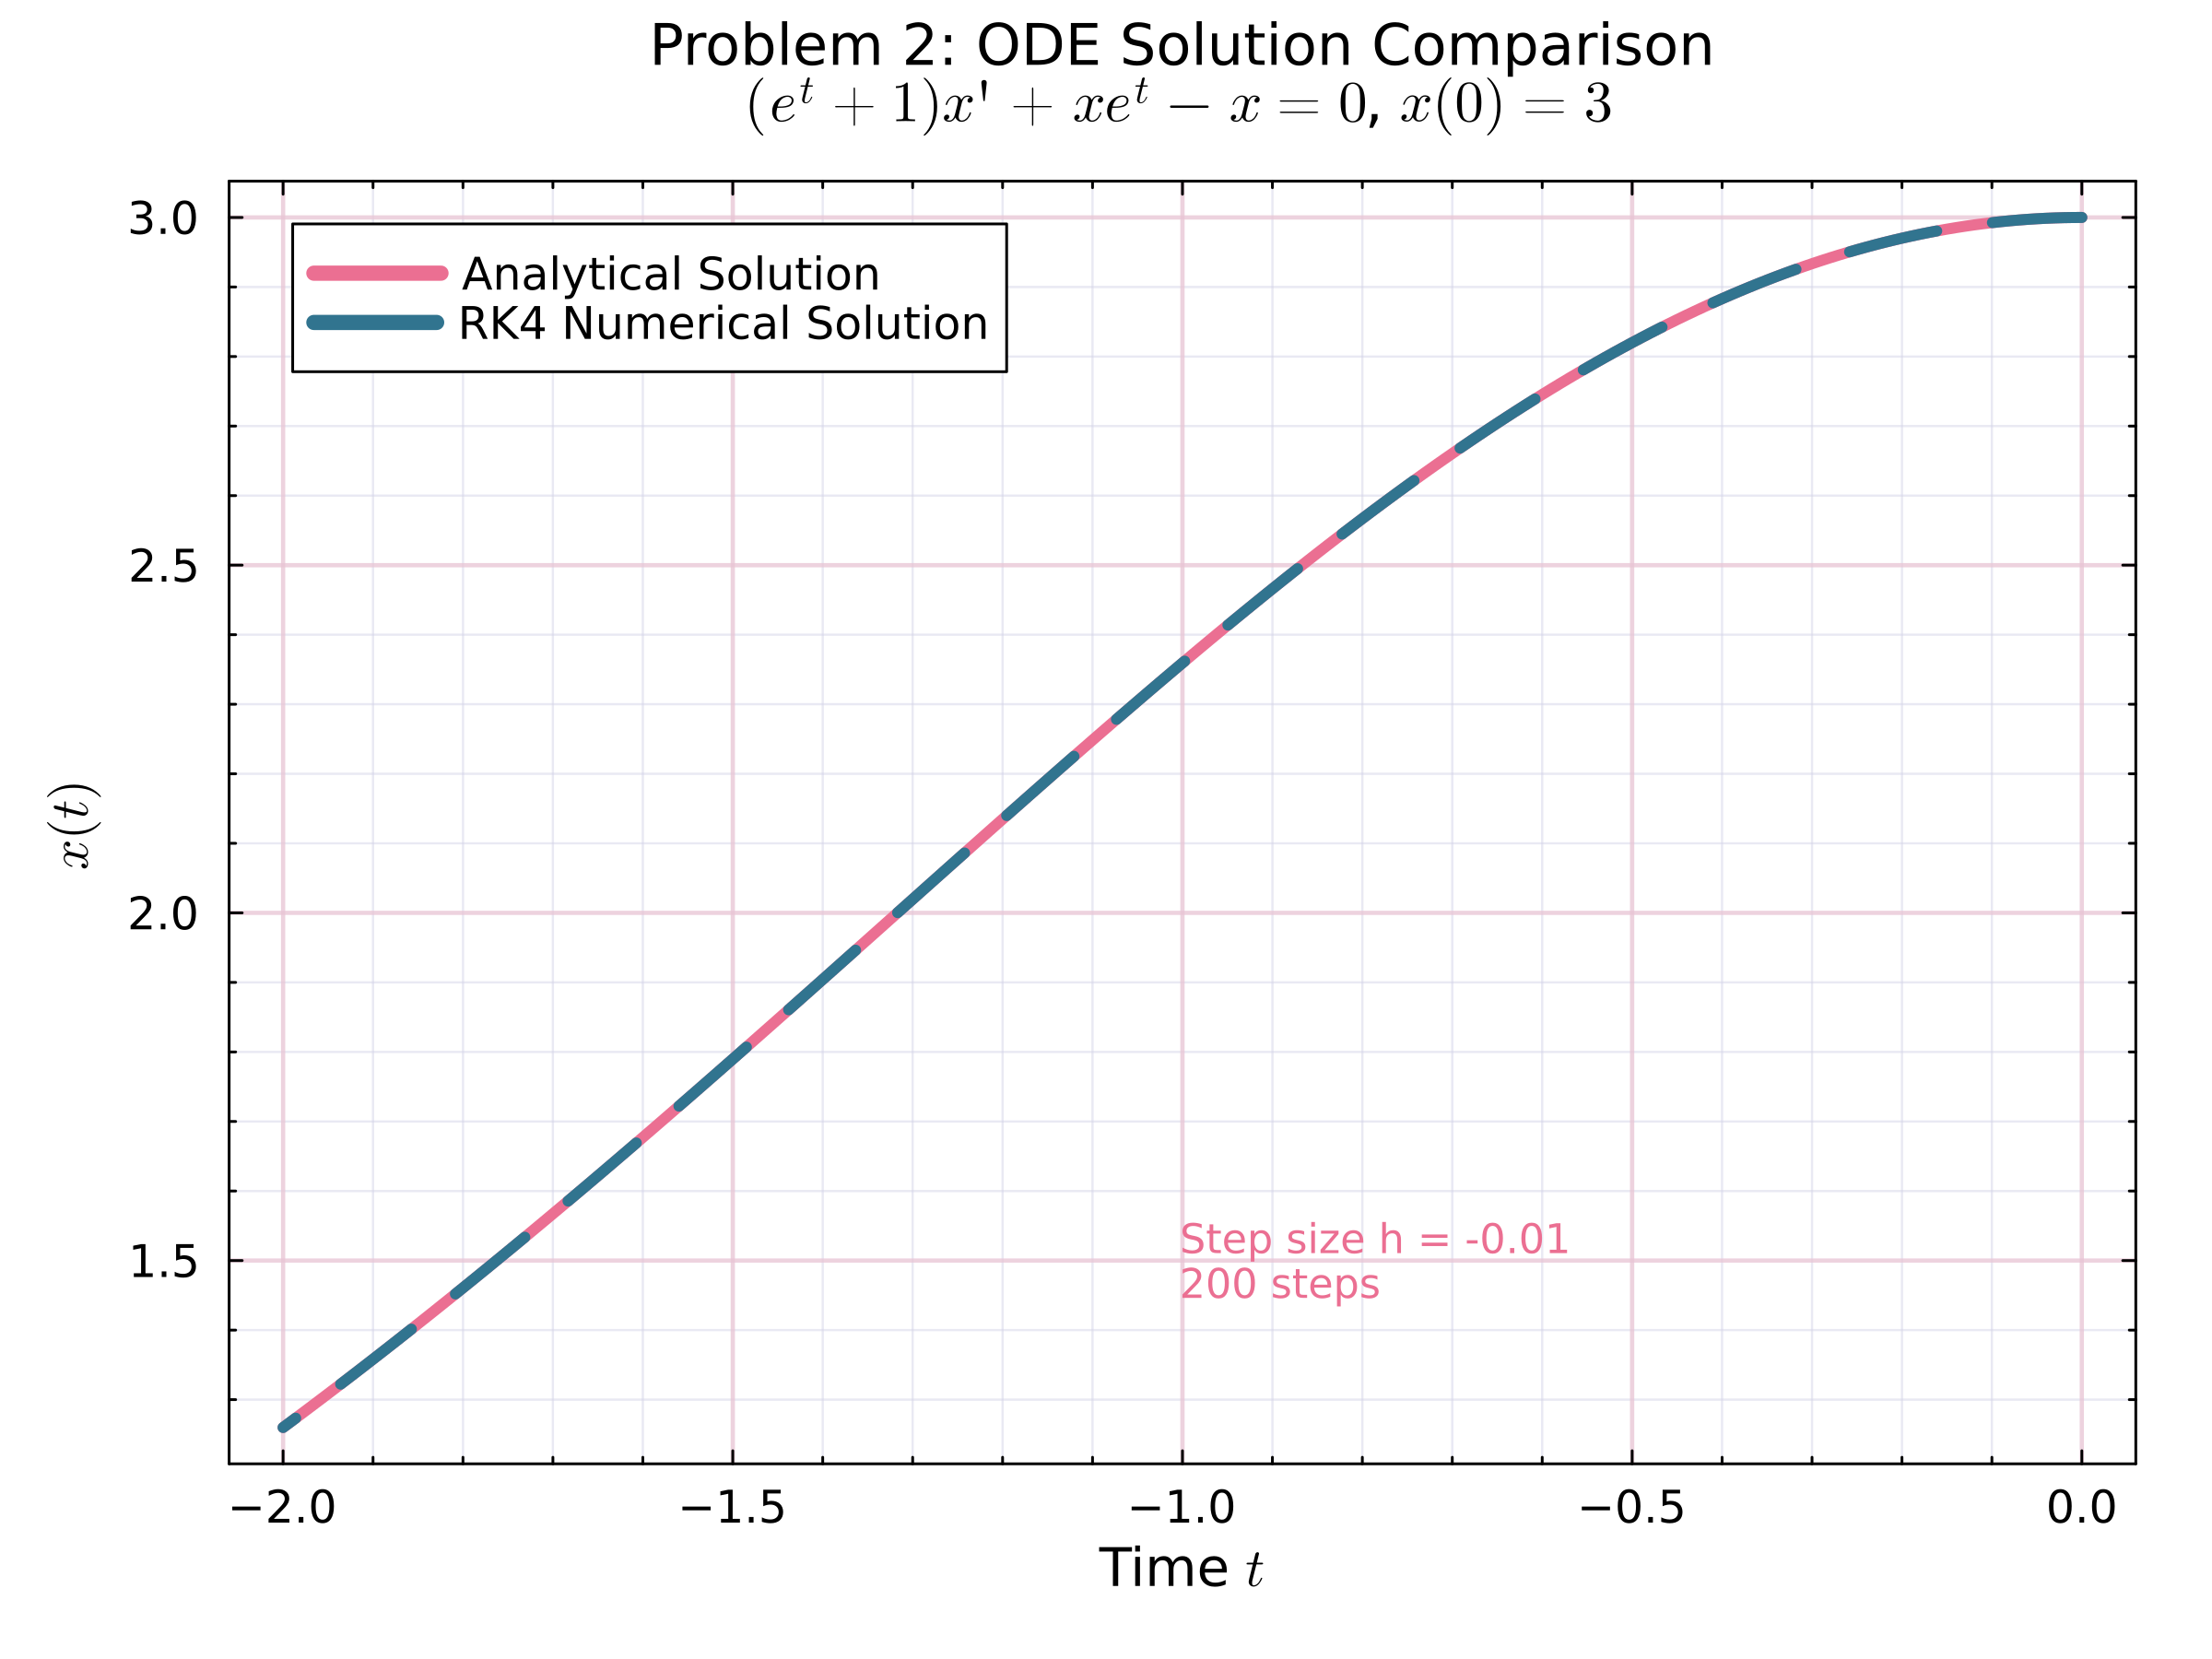
\includegraphics[width=0.85\textwidth]{figures/p02_trajectory_comparison.png}
\caption{Comparison of RK4 numerical solution (dashed blue line) with analytical solution (solid pink line) for the ODE $(e^t + 1)x' + xe^t - x = 0$ with $x(0) = 3$. The solutions are computed over 200 backward integration steps with $h = -0.01$.}
\label{fig:p02_trajectory}
\end{figure}

\vspace{2em}
\noindent\rule{\textwidth}{0.4pt}

\clearpage
\subsection*{Conclusion}
\addcontentsline{toc}{subsection}{Conclusion}

\textbf{Error Analysis:}
\begin{itemize}
    \item Maximum absolute error: $1.107 \times 10^{-11}$
    \item Mean absolute error: $2.144 \times 10^{-12}$
\end{itemize}

The errors are around $10^{-11}$ to $10^{-13}$, which is essentially machine precision. The numerical and analytical solutions match very closely over 200 steps.

\textbf{Verification:} Results checked against Wolfram Alpha \cite{wolframalpha_rk4_verification}.

\vspace{2em}
\noindent\rule{\textwidth}{0.4pt}
